\begin{frame}{Arquitecturas de Hardware}
    Procesadores
    
    \vspace{1cm} Arquitecturas
    \begin{itemize}
        \item RISC
        \item CISC
    \end{itemize}
    
    \vspace{1cm}Pipelines
\end{frame}

\begin{frame}{Arquitecturas de Memoria}
    \begin{columns}
        \column{.7\textwidth}
        \begin{block}{ROM -- \emph{Read Only Memory}}
            \begin{itemize}
                \item ROM    $\Rightarrow$ Se graban los datos durante la fabricación, el menor costo
                \item PROM   $\Rightarrow$ \emph{Programmable ROM}: Se puede grabar solo una vez
                \item EPROM  $\Rightarrow$ \emph{Erasable PROM}: Se puede borrar con luz ultravioleta y volver a grabar (varios ciclos)
                \item EEPROM $\Rightarrow$ \emph{Electric EPROM}: Se puede grabar y borrar varios ciclos sin necesidad de desmontar del hardware
            \end{itemize}
        \end{block}
        \column{.25\textwidth}
        \begin{block}{EPROM}
            \begin{center}
                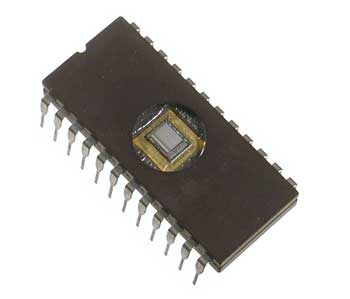
\includegraphics[width=.9\linewidth]{../imagenes/eprom}
            \end{center}
        \end{block}
    \end{columns}
\end{frame}

\begin{frame}{Arquitecturas de Memoria}
    \begin{columns}
        \column{.6\textwidth}
        \begin{block}{RAM -- \emph{Random Access Memory}}
            \begin{itemize}
                \item \emph{Dynamic} RAM (DRAM) $\Rightarrow$ Económica y bajo consumo porque se basa en capacitores, requiere un ciclo de refresco
                \item \emph{Static} RAM (SRAM) $\Rightarrow$ Más eficiente pero de mayor consumo porque se basa en transistores
            \end{itemize}
        \end{block}
        \column{.35\textwidth}
        \begin{block}{DRAM}
            \begin{center}
                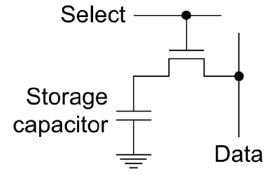
\includegraphics[width=.9\linewidth]{../imagenes/dram}
            \end{center}
        \end{block}
        \begin{block}{SRAM}
            \begin{center}
                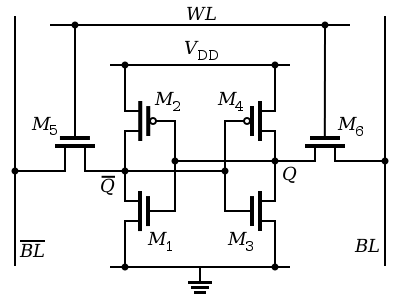
\includegraphics[width=.9\linewidth]{../imagenes/sram}
            \end{center}
        \end{block}
    \end{columns}
\end{frame}

\begin{frame}{Arquitecturas de Memoria}
    \begin{block}{Memoria Caché}
        \begin{center}
            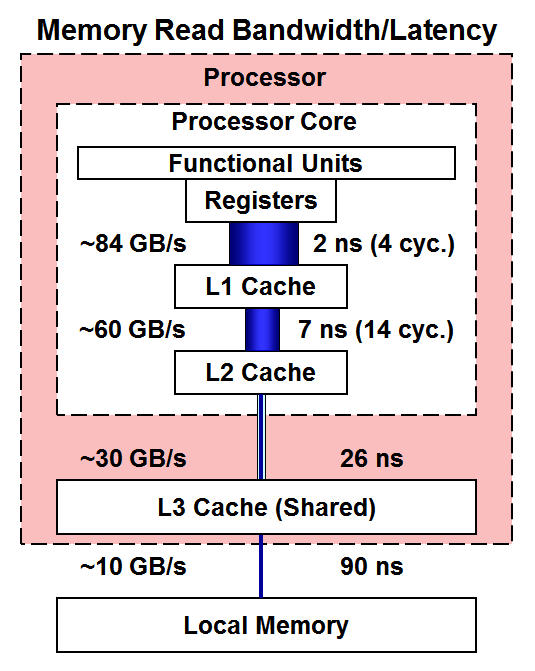
\includegraphics[width=.5\linewidth]{../imagenes/memLevels}
        \end{center}
    \end{block}
\end{frame}

\begin{frame}{Arquitecturas de Memoria}
    \begin{block}{Memoria Caché}
        \begin{center}
            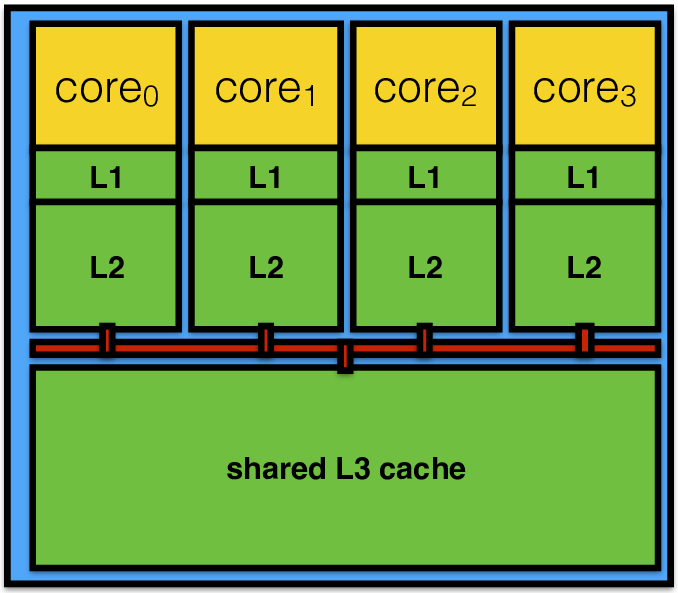
\includegraphics[width=.7\linewidth]{../imagenes/CPUcache}
        \end{center}
    \end{block}
\end{frame}

\begin{frame}{Representación de los Números}
    Representación de Números
    \begin{itemize}
        \item Enteros $\Rightarrow$ Subconjunto de $\mathbb{Z}$
        \item Reales $\Rightarrow$ Subconjunto de $\mathbb{R}$
        \begin{itemize}
            \item Existen varios formatos para representarlos
            \begin{itemize}
                \item Punto fijo
                \item Punto Flotante
                \item BCD (\emph{Binary Coded Decimal})
                \item Fracción entre Enteros
                \item \dots
            \end{itemize}
            \item Varía precisión y tiempo de procesamiento
        \end{itemize}
    \end{itemize}
\end{frame}

\begin{frame}{Números Punto Flotante -- IEEE 754}
    \begin{block}{Ventajas}
        \begin{itemize}
            \item Estándar utilizado en general
            \item Especifica:
            \begin{itemize}
                \item Cómo representarlos
                \item Cómo operar
            \end{itemize}
            \item Ampliamente difundido para propósito general
            \item Implementación por software o hardware (co--procesador)
        \end{itemize}
    \end{block}
    \begin{block}{Desventajas}
        \begin{itemize}
            \item Distribución no uniforme
            \item Presenta problemas de precisión para usos específicos
            \item Las optimizaciones del compilador reducen precisión
        \end{itemize}
    \end{block}
\end{frame}